% mainfile: ../../main.tex
\chapter{Characterization of the cryostat performance}\label{ch:setup:cooling}
\AutoLettrine{An} essential feature of the confocal microscope discussed in \thethesis is its capability to perform optical measurements at Millikelvin temperatures.
As individual quantum systems are singled out for applications in quantum technology, thermal excitations with energy $\kb T = \qty{86}{\micro\eV\per\kelvin}\times T$ quickly become the dominating energy scale and overshadow the desired effects.
Hence, typical energies in the solid state on the \unit{\micro\eV} scale, such as Zeeman energies of individual spins with energy $\mub B = \qty{58}{\micro\eV\per\tesla}\times B$, require temperatures well below \qty{1}{\kelvin} to suppress thermal excitations.

By design the \odin dry \gls{dr} housing the microscope is rated for base temperatures at the mixing chamber plate below $\Tmxc=\qty{10}{\milli\kelvin}$.
However, several factors, both passive and active, introduce additional heat loads that can potentially raise the base temperature if too large:
\begin{enumerate}
    \item \label{itm:setup:cooling:wiring}
    DC and RF wiring.
    These introduce thermal links between the sample and higher temperature stages as well as add noise that raises the electron temperature in the sample.
    \item \label{itm:setup:cooling:positioners}
    Wiring and operation of the \positioner nanopositioners.
    The nanopositioners require special low-impedance connections to ensure a large enough bandwidth for the stick-slip mode of operation.
    Moreover, the resistive position readout introduces additional heating.
    \item \label{itm:setup:cooling:optical}
    Optical access.
    The free-space optical access requires a direct \gls{los} port to the sample.
    This inevitably allows infrared radiation from room temperature into the cryostat, something that is usually painstakingly prevented when designing a cryostat.
    Furthermore, optical experiments involve irradiating the sample with a highly focused laser beam, some of which will be absorbed and contribute to heating.
\end{enumerate}

In this chapter, I characterize the cooling performance of the dry \gls{dr} housing the microscope in various ways. % TODO: wishy-washy
I first discuss the cooling power in terms of the base temperature \Tmxc reached for different configurations in \cref{sec:setup:cooling:power}.
This is often quoted as the bath, lattice, or \emph{phonon} temperature,\sidenote{
    This terminology can be misleading as the phonon temperature can also be measured with a quantum transport device, which will most likely see a different phonon temperature than the thermometer on the mixing chamber plate because of a temperature gradient between the heating source close to the sample and sink (the mixing chamber) close to the thermometer.
}
and can be read out using the resistive \ch{RuO_2} thermometry setup installed in the \gls{dr}.
Then, in \cref{sec:setup:cooling:etemp}, I present measurements of the \emph{electron} temperature, a quantity that is arguably more expressive of the cryostat's capability to perform precise measurements as it is more sensitive to, for example, electrical noise introduced by the wiring.

\section{Cooling power}\label{sec:setup:cooling:power}
The base temperature (\Tmxc) can be read out from the resistance bridge connected to the gas handling PC controlling the cryostat.
Two different thermometers are installed on the mixing chamber, a Cernox\textsuperscript{\textregistered} sensor that works in the range from room temperature down to around \qty{2}{\kelvin} for cooldown, and a \ch{RuO_2} sensor that works from \qty{30}{\kelvin} down to, in principle, zero for base temperature operation.
The resistance bridge performs a four-terminal measurement of the sensor resistance and converts it to a temperature according to a sensor-specific calibration $\Tmxc(R_{\ch{RuO_2}})$.
Since the particular sensor installed in our system was only calibrated down to \qty{30}{\milli\kelvin}, I had to extrapolate the calibration curve as the system reaches lower temperatures than this, and hence the temperatures below this threshold quoted here are not guaranteed to be correct.

\begin{marginfigure}
    \centering
    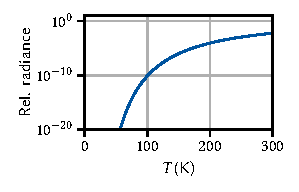
\includegraphics{img/pdf/setup/black_body_radiance}
    \caption[\imgsource{img/py/setup/cooling_power.py}]{
        Relative black-body radiance obtained by integrating \cref{eq:setup:cooling:blackbody} from $\lambda = \qtyrange{0}{4.5}{\micro\meter}$ and normalizing to the total radiance.
        At $T=\qty{300}{\kelvin}$, the fraction of total radiance residing in the high-energy part of the spectrum is still only \qty{0.6}{\percent}.
    }
    \label{fig:setup:cooling:blackbody}
\end{marginfigure}

With the configuration described in \citer{Descamps2021}, the \gls{dr} reached a base temperature of $\Tmxc = \qty{30}{\milli\kelvin}$.
This included all DC and RF wiring as well as a single \gls{ar}-coated window sealing the vacuum space on top of the fridge for optical access.
To investigate the influence of ambient thermal radiation entering the cryostat through the optical access port, or, more generally, radiation from the higher- to lower-temperature stages, I measured the base temperature for two additional configurations; once with an additional \gls{ar}-coated window inserted into the optical path on the Cold plate, and once with three windows installed on the \gls{pt1}, \gls{pt2}, and Still plates.
The windows (\thewindow) are made from UV fused silica with \gls{ar} coating\sidenote{
    Depending on the manufacturer, the coating for the range \qtyrange{650}{1050}{\nano\meter} is called \acrshort{bbar} VIS-\acrshort{nir} or \acrshort{bbar}-B.
}
The manufacturer quotes a typical reflectance of \qty{0.25}{\percent} in the relevant wavelength range, while the glass is largely transmissive for wavelengths below $\lambda_{\mr{cutoff}}\sim\qty{4.5}{\micro\meter}$.
Since the spectral radiance of thermal black-body radiation~\cite{Planck1900}
\begin{equation}\label{eq:setup:cooling:blackbody}
    B_\lambda(\lambda, T) = \frac{2 h c^2}{\lambda^5}\frac{1}{\exp(\flatfrac{hc}{\lambda\kb T}) - 1}
\end{equation}
is small up to $\lambda_{\mr{cutoff}}$ at low ($\leq\qty{300}{\kelvin}$) temperatures as shown in \cref{fig:setup:cooling:blackbody}, we expect the windows be largely opaque to thermal radiation and hence be quite effective in reducing the radiative heat load.
As the radiative power scales with $T^4$ and there is at the same time more cooling power available at higher-temperature stages, installing windows there result in an overall better performance.

\begin{margintable}
    \centering
    \footnotesize
    \caption{
        \Gls{mxc} temperature for different configurations of \gls{ar} coated windows (\thewindow) inside the \gls{dr}.
    }
    \label{tab:setup:cooling:windows}
    \begin{tabular}{lr}
        \toprule
        \textsc{Windows}                      & $T_\mathrm{\acrshort{mxc}}$ \textsc{(mK)} \\
        \midrule
        None                                  & 30.0                                      \\
        Cold                                  & 11.0                                      \\
        \acrshort{pt1}, \acrshort{pt2}, Still & 7.9                                       \\
        \bottomrule
    \end{tabular}
\end{margintable}

\Cref{tab:setup:cooling:windows} shows the measured mixing chamber temperatures for the different window configurations.
Indeed, already a single window installed on the Cold plate significantly reduces the base temperature.
While the windows do introduce additional reflections of the laser spot when imaging the sample due to the finite remaining reflectance, their intensity is low enough, and their position on the camera far enough away from the main spot to be an issue.
On the contrary, their presence can be quite useful when aligning the laser spots from the two arms of the optical head by aligning them in such a way that the reflections overlap.

\todo{I / we, general rephrasing}
Besides the ambient radiation, there is also the heat load introduced by the partial absorption of the laser excitation during optical measurements.
In order to characterize both the heat load and measure the absorptance $A$ of our sample, I irradiated a flip-chip-bonded membrane sample such as measured in \cref{part:exp} with the laser at \qty{815}{\nano\meter} and measured the increase in base temperature.
The sample consists of a \qty{220}{\nano\meter} thick \ch{GaAs/AlGaAs} membrane glued with epoxy to a \ch{Si} host substrate chip for handling.
As the samples are flip-chip bonded, light that is transmitted through the chip without being absorbed or reflected will then hit the surrounding puck and scatter.
Thus, to be precise, I measured $A+T$ this way, where $T$ is the transmittance, assuming that light that exits the membrane will be absorbed \emph{somewhere} and contribute to heating.
I will nonetheless refer to the measured quantity as simply $A$.

With the power meter mounted in the transmission direction of the excitation arm of the optical head (\cf \cref{fig:setup:optics:optical_path}), I measured the amount of power directed towards the sample by scaling the measured power with the ratio of transmittance and reflectance of the \gls{bs}, $T\div R\approx\num{15}$.
Assuming negligible losses on the way towards the sample, I then recorded the mixing chamber temperature as function of laser power.
To relate that change in temperature to a heat load $\dot{Q}$ deposited on the sample, I calibrated the cooling power of the \gls{dr} using the built-in heaters.
Setting a heater power and waiting for the mixing chamber temperature to settle thus yields the cooling power $P_{\mr{cool}}$ as function of temperature \Tmxc, which is expected to follow the quadratic relationship~\cite{DeWaele2011}
\begin{equation}\label{eq:setup:cooling:dr_power}
    P_{\mr{cool}} = \dot{Q} = \alpha \Tmxc^2 + \beta.
\end{equation}
As a last step, we can use a simple model of absorption of the laser on the sample in thermal equilibrium,
\begin{equation}\label{eq:setup:cooling:absorptance}
    P_{\mr{cool}} = P_{\mr{nr}} = A P_{\mr{laser}},
\end{equation}
where $P_{\mr{nr}}$ is the amount of power deposited into nonradiative emission channels causing heating of the lattice, to relate the incident laser power $P_{\mr{laser}}$ to the cooling power and thus obtain the absorptance $A$.

\begin{marginfigure}
    \centering
    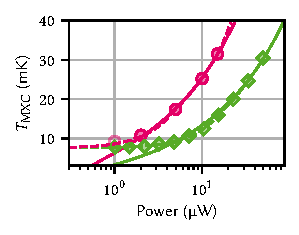
\includegraphics{img/pdf/setup/laser_heating}
    \caption[\imgsource{img/py/setup/cooling_power.py}]{
        \Acrlong{mxc} temperature as function of heater (magenta) and laser (green) power.
        Solid lines are fits to \cref{eq:setup:cooling:dr_power} including only the solid markers.
        Green dashed line is a quadratic smoothing spline fit to all laser data points.
        Magenta dashed line is the laser spline scaled to match the heater data with fitted factor $A=\qty{28}{\percent}$ corresponding to the fraction of laser power absorbed and non-radiatively emitted.
    }
    \label{fig:setup:cooling:laser}
\end{marginfigure}

\Cref{fig:setup:cooling:laser} shows data sets obtained with the \gls{mxc} heater (magenta) and laser (green).
The solid lines are fits to \cref{eq:setup:cooling:dr_power} including the solid data points only as at low powers there is clearly a deviation from the square-root relationship between the two.
Comparing the fit results for $\alpha$, we obtain $A = \qty{28.5}{\percent}$.
Alternatively, we can fit a quadratic smoothing spline to the laser data (magenta dashed line) and fit a version scaled according to \cref{eq:setup:cooling:absorptance} to the heater data (green dashed line).
This yields $A = \qty{28.1}{\percent}$ in good agreement to the value obtained from fitting the theoretical model.
Furthermore, the data shows that only at laser powers above \qty{10}{\micro\watt} the \gls{mxc} heats up appreciably.

Lastly, let us address the impact of the \positioner position readout.
The nanopositioners are crucial in the operation of the microscope as they are used to position the sample with respect to the focal spot of the objective lens.
They operate in slip-stick mode which naturally generates heat through friction when moving.
However, the resistive position readout also contributes to heating, so in order to assess if the readout should be switched off when it is not required to avoid unnecessarily elevated cryostat temperatures, I measured \Tmxc as a function of readout voltage.
Note that the \positionercontroller piezo controller offers the option of lock-in measurement for readout, which should be enabled as it improves the \gls{snr} and thus allows for a smaller readout voltage $V_{\mr{AC}}$.

\begin{marginfigure}
    \centering
    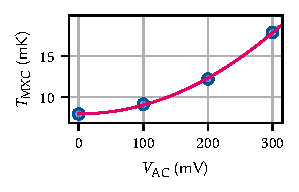
\includegraphics{img/pdf/setup/anc_readout_heating}
    \caption[\imgsource{img/py/setup/cooling_power.py}]{
        \Acrlong{mxc} temperature as function of nanopositioner AC readout voltage.
        The secondary axis indicates the conversion from $T_{\mr{\acrshort{mxc}}}$ to power obtained in \cref{fig:setup:cooling:laser} which is approximately linear in this regime, leading to the expected $P\sim R\inverse V_{\mr{AC}}^2$ behavior.
        Solid line is a fit to the power with $R=\qty{16.9}{\kilo\ohm}$.
    }
    \label{fig:setup:cooling:anc}
\end{marginfigure}

\Cref{fig:setup:cooling:anc} shows the temperature as function of $V_{\mr{AC}}$, as well as the equivalent power from the calibration performed in \cref{fig:setup:cooling:laser}.
The expected Ohmic behavior is evident, resulting in a resistance of $R=\qty{16.9}{\kilo\ohm}$.
We can conclude that for $V_{\mr{AC}} < \qty{100}{\milli\volt}$, heating from the positioner readout is negligible, which is a regime where the \gls{snr} of the measurement is reasonable.

\section{Electron temperature}\label{sec:setup:cooling:etemp}
In the previous section, I discussed various sources of heating of the cryostat temperature measured at the mixing chamber plate using a commercial resistive thermometer.
An arguably more relevant metric for quantum device experiments is the electronic temperature which -- depending on how it is measured in detail -- corresponds to the temperature of the Fermi distribution of electrons in or coupled to a reservoir rather than the temperature of the crystal lattice.
Precisely because the behavior of these quantum devices depends so sensitively on the electron temperature, one can also flip this relationship on its head and use them to \emph{measure} the temperature, an instance of single controlled quantum systems being used as highly sensitive probes of physical quantities known as \emph{quantum sensing}~\cite{Degen2017}.
\Glspl{gdqd} hosted in the \gls{2deg} of a semiconductor heterostructure offer several different ways of measuring the electron temperature that are each different in subtle ways.
For example, using an adjacent charge sensor, one can measure the width of a lead\sidenote{
    A \enquote{lead} is a reservoir of charge carriers coupled to a quantum dot.
}
transition~\cite{Maradan2014} or the width of the inter-dot transition in a double \gls{qd}~\cite{DiCarlo2004}.
Simpler still, one can measure the width of a Coulomb resonance in the conductance through a \gls{qd}~\cite{Ihn2009,Maradan2014}.
All of these methods rely on some form of energy reference scale that relates the energy of an electron confined in a \gls{qd} to some externally controlled parameter such as a voltage, however.
Typically this is the so-called \emph{lever arm} $\alpha$, which is the constant of proportionality between the plunger gate voltage and the electrochemical potential $\mu_N$ for adding the $N$th electron to the quantum dot~\cite{Ihn2009}.
It can be measured using pulsed-gate spectroscopy~\cite{Fujisawa2001,Harbusch2010}, photon-assisted tunneling~\cite{Kouwenhoven1994}, or using bias spectroscopy (Coulomb diamonds)~\cite{Kouwenhoven2001,Ihn2009}.

\begin{marginfigure}
    \centering
    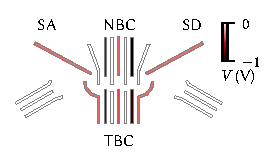
\includegraphics{img/pdf/setup/diamonds_gl}
    \caption[\imgsource{img/py/setup/transport.py}]{
        Gate layout of a quadruple \acrlong{qd} with two charge sensor \glspl{qd} from \citer{Cerfontaine2019}.
        Ohmic contacts used for transport measurements are right (left) of SA (SD).
        The gates are colored according to the voltages applied with the device hosting a single large \gls{qd} in the few-electron, sequential tunneling regime.
    }
    \label{fig:setup:cooling:etemp:gl}
\end{marginfigure}

Here, I chose the simplest of these techniques that require the least tune-up to avoid unnecessarily complicating things.
That is, I formed a single \gls{qd} in a gated \ch{GaAs/AlGaAs} heterostructure and extracted the lever arm from Coulomb diamonds and the electron temperature from the conductance trace of a Coulomb resonance at zero bias in the sequential tunneling regime.
The gate layout of the device used is shown in \cref{fig:setup:cooling:etemp:gl}.
Designed for two-qubit experiments with two-electron spin qubits by \citet{Cerfontaine2019}, I tuned the device to host a single large \gls{qd} in the center of the device.
The gates are color-coded according to the voltages applied with the device in the few-electron regime.
I applied a bias voltage at the Ohmic contact situated to the right of gate SA using a \decadac voltage source and measured the current at the Ohmic contact to the left of gate SD using a \baseltia I/V converter with non-inverting input shorted to ground.\sidenote{
    I use the same naming scheme for gate electrodes as \citer{Cerfontaine2019}.
}
Gate voltages were also supplied by the \decadac, divided by six and low-pass filtered at room temperature in the \gls{bob}.
All but the four long gates (RFA--RFD) coming in from the top of the device were connected to the filtered DC lines as described in \citer{Descamps2021}.
The former were connected to RF lines attenuated with \qtylist{20;6;0;3}{\decibel} attenuators mounted to the \gls{pt2}, Still, Cold, and \gls{mxc} plates, respectively, and connected to a \hdawg but unused during these experiments.

To tune the electrochemical potential in the dot, I set up a virtual plunger gate~\cite{Botzem2018} from a linear combination of the gates NBC and TBC by performing a two-dimensional sweep of TBC against NBC\@.
From the slope $m$ of a charge transition in the voltage space spanned by TBC and NBC, I computed the weights of the virtual gate in terms of the physical gates as
\begin{equation}
    V_{\mr{p}} = \frac{1}{\sqrt{1 + m^2}}\left(\mr{TBC} + m\times \mr{NBC}\right).
\end{equation}
Following this procedure, even a dot that does not lie in the middle between the two gates, \ie, couples more strongly to one than the other gate, should not move in position when changing the virtual gate voltage.
Having set up the virtual plunger gate, I performed a Coulomb diamond measurement wherein the (virtual) plunger gate is swept as the source-drain bias voltage is varied~\cite{Ihn2009}.\sidenote{
    In this case, the source-drain bias is asymmetric as the drain is always grounded and only the electrochemical potential of the source reservoir is changed.
    This does not qualitatively change the physics of the measurement, though.
}
The left panel of \cref{fig:setup:cooling:etemp:diamonds} shows the current of the Coulomb diamond measurement.
Starting from zero bias, when current can only flow through the Coulomb-blockaded \gls{qd} when both source and drain are aligned with an energy level in the dot, increasing the bias voltage opens up the \emph{bias window}, allowing current to flow as long as the dot's energy level is inside the window.
This defines areas of zero (blockaded) current within the space of plunger and bias voltage that takes on the shape of a diamond whose height (along the bias axis) is given by the energy penalty of adding another electron to the dot~\cite{Ihn2009},
\begin{equation}
    E_\mr{add} = \mu_{N+1} - \mu_N = E_c + \Delta E,
\end{equation}
where $\mu_N$ is the electrochemical potential of the dot with $N$ electrons, $E_c$ is the charging energy due to Coulomb repulsion, and $\Delta E$ is the single-particle energy spacing.
At the same time, the width of a diamond (along the gate voltage axis) is given by
\begin{equation}
    \Delta V_{\mr{p}} = \alpha\inverse E_\mr{add},
\end{equation}
implying that we can extract the lever arm $\alpha$ from the geometry of the diamonds.
Drawing lines with slopes $m_1$ and $m_2$ along the onsets and offsets of current through the Coulomb resonance at zero bias (dashed gray lines), I obtained
\begin{equation}
    \alpha = \abs{\Delta m} = \abs{m_1 - m_2} \approx\qty{0.11}{\eV\per\volt}.
\end{equation}

\begin{figure*}
    \centering
    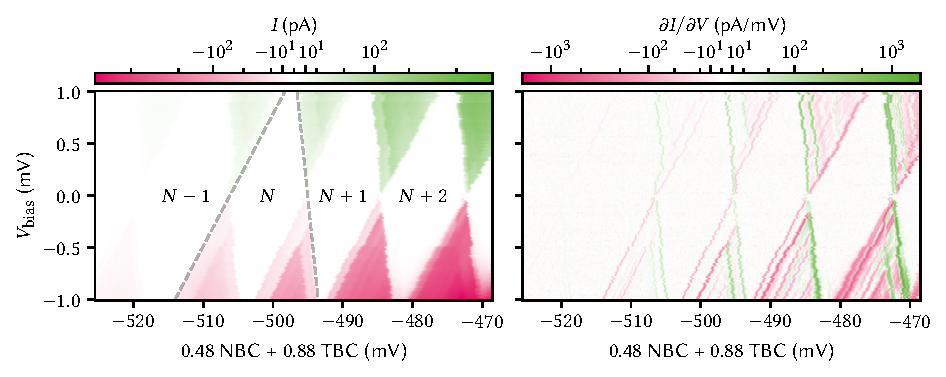
\includegraphics{img/pdf/setup/diamonds}
    \caption[\imgsource{img/py/setup/transport.py}]{
        Coulomb diamond measurement of the single \gls{gdqd} confined by applying static voltages to the gates shown in \cref{fig:setup:cooling:etemp:gl}.
        The left panel shows the current measured with a \gls{tia} with a bias applied on one side of the device.
        The horizontal axis shows the virtual plunger gate swept for each bias voltage indicated on the vertical axis.
        The difference in slope of the dashed gray lines around the $N$-electron diamond yields the lever arm $\alpha$ converting virtual plunger gate voltage to (relative) energy inside the dot.
        From the fact that the slopes are not equal up to a sign we can infer that the coupling to source and drain reservoirs is unequal also, indicating that either the dot is situated closer to SA than to SD, or the topology of the tunneling contacts in the \gls{2deg} is different due to different electrostatic potential.
        The right panel shows the differential conductance obtained from differentiating the data from the left panel along the plunger gate axis.
        Clearly visible are several additional transition lines which correspond to excited states inside the dot becoming energetically available within the bias window.
    }
    \label{fig:setup:cooling:etemp:diamonds}
\end{figure*}

Although not of particular interest for the electron temperature, a Coulomb diamond measurement can also be used for excited state spectroscopy.
Computing the differential conductance $\partial I/\partial V_{\mr{p}}$ makes visible a host of additional transition lines in the conducting region of the map (right panel of \cref{fig:setup:cooling:etemp:diamonds}).\sidenote{
    Features inside the blockaded region can also occur, indicative of co-tunneling.
}
These correspond to excited states of the quantum dot entering the bias window.
Their sign depends on the tunnel coupling of the state to source and drain~\cite{Ihn2009}.

\begin{marginfigure}
    \centering
    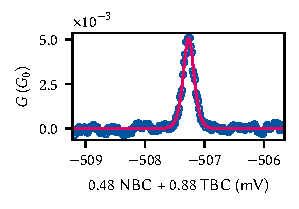
\includegraphics{img/pdf/setup/coulomb_resonance}
    \caption[\imgsource{img/py/setup/transport.py}]{
        Conductance of a Coulomb resonance in the sequential tunneling regime.
        Magenta line is a fit to \cref{eq:setup:cooling:etemp:resonance} with $T = \qty{74.9}{\milli\kelvin}$ and $\Gamma = \qty{0.524+-0.005}{\micro\eV}$.
    }
    \label{fig:setup:cooling:etemp:resonance}
\end{marginfigure}

Having measured the energy reference scale, the lever arm $\alpha$, I proceeded to measure the conductance through a single Coulomb resonance as function of virtual plunger gate voltage $V_{\mr{p}}$ in order to measure the electron temperature.
The line shape of such a resonance is qualitatively different in two limiting regimes of two competing energy scales, the tunnel coupling $\Gamma$ of the quantum dot to the leads and the thermal energy $\kb T$.
If the former dominates transport through the \gls{qd} is said to be in the resonant (coherent) tunneling regime while if the latter dominates, it is said to be in the sequential (incoherent) tunneling regime~\cite{Ihn2009}.
For resonant tunneling, the line shape has the form of a Lorentzian of width $\Gamma$.
For sequential tunneling, the line shape of a resonance at $V_{\mr{p}}^{\mr{res}}$ is given by
\begin{equation}\label{eq:setup:cooling:etemp:resonance}
    G(V_{\mr{p}}) = \frac{e^2}{2h}\frac{\Gamma}{4\kb T}\cosh^{-2}\left[\frac{\alpha\left(V_{\mr{p}} - V_{\mr{p}}^{\mr{res}}\right)}{2\kb T}\right]
\end{equation}
in linear response (small bias).
Thus, I tuned the device to small tunnel couplings (high tunnel barriers) and measured $G(V_{\mr{p}})$ with a small bias voltage.
The resulting conductance trace is shown in \cref{fig:setup:cooling:etemp:resonance} together with a fit to \cref{eq:setup:cooling:etemp:resonance}.
From the fit we can extract the parameters $T = \qty{74.9}{\milli\kelvin}$ and $\Gamma = \qty{0.524+-0.005}{\micro\eV} = \qty{6.08+-0.06}{\milli\kelvin}$, confirming the sequential tunneling regime of $\Gamma\ll\kb T$.\sidenote{
    In a different tuning state of the device, the conductance would also sometimes change sign close to the resonance at small biases.
    The line shape in this configuration was well described by source and drain reservoirs at different temperatures,
    \begin{equation*}
        G(V_{\mr{p}}) \propto f(V_{\mr{p}} - V_{\mr{p}}^{\mr{res,S}}) - f(V_{\mr{p}} - V_{\mr{p}}^{\mr{res,D}}),
    \end{equation*}
    with the Fermi-Dirac distribution
    \begin{equation*}
        f(V) = \left[\exp(\alpha V/\kb T) + 1\right]\inverse.
    \end{equation*}
    The precise physical mechanism behind this behavior is not understood.
}
